\begin{problem}[问题6.5]
直角域内$z_0$点存在强度为$\Gamma$的点涡, 求其复速度势.
\end{problem}

\begin{solution}
\begin{multicols}{2}
\textbf{解:} 利用镜像法, 分别以实轴虑轴为边界, 在$z_0$的对称点引入相应的点涡, 如图\ref{fig:RectPointVortex}所示. 则有
\begin{eqnarray}
W(z) &=& +\frac{\Gamma}{2\pi i}\ln(z-z_0) -\frac{\Gamma}{2\pi i}\ln(z-\overline{z_0})\nonumber\\
     & & -\frac{\Gamma}{2\pi i}\ln(z+\overline{z_0})+\frac{\Gamma}{2\pi i}\ln(z+z_0)\nonumber\\
     &=& \frac{\Gamma}{2\pi i}\ln\Big[\frac{z^2-z_0^2}{z^2-\overline{z_0}^2}\Big]\nonumber
\end{eqnarray}

\vspace{0.1em}
\begin{center}
\usetikzlibrary{%
    decorations.pathreplacing,%
    decorations.pathmorphing,arrows
}
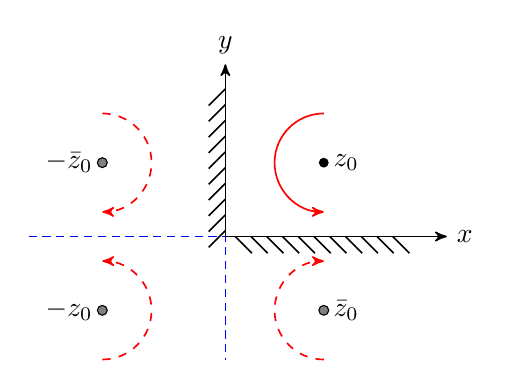
\begin{tikzpicture}[ media/.style={font={\footnotesize\sffamily}},
    interface/.style={
        postaction={draw,decorate,decoration={border,angle=-45,
                    amplitude=0.3cm,segment length=2mm}}},scale=1.25]
\draw[semithick,interface](1,1.5)--(1,0)--(3,0);
\draw[semithick,->,>=stealth'](3,0)--(3.25,0) node[right]{$x$};
\draw[semithick,->,>=stealth'](1,1.5)--(1,1.75) node[above]{$y$};
\draw[semithick,blue,densely dashed](-1,0)--(1,0)--(1,-1.25);

\fill(2,0.75) circle(0.05) node[right]{$z_0$};
\draw[semithick,red,->,>=stealth'](2,1.25) arc(90:270:0.5);
\fill[gray,draw=black](-0.25,0.75) circle(0.05) node[left,black]{$-\bar{z}_0$};
\draw[semithick,red,->,>=stealth',dashed](-0.25,1.25) arc(90:-90:0.5);

\fill[gray,draw=black](-0.25,-0.75) circle(0.05) node[left,black]{$-z_0$};
\draw[semithick,red,->,>=stealth',dashed](-0.25,-1.25) arc(-90:90:0.5);

\fill[gray,draw=black](2,-0.75) circle(0.05)node[right,black]{$\bar{z}_0$};
\draw[semithick,red,->,>=stealth',dashed](2,-1.25) arc(-90:-270:0.5);

%\fill[blue!20](0.5,1)--(0.5,0.05)--(2,0.05)--(2,0.75);

%\draw[semithick] (0.5,1.25)--(0.5,0.05)--(2,0.05)--(2,1.25);
%\draw[blue, semithick] (0.5,1)--(2,0.75);
%\draw[blue,dashed](2,0.75)--(0.75,0.75);
%\draw (1,0.75) arc(180:170:1) node[blue,above]{$\theta$};
%\draw [semithick,->,>=stealth',blue] (2.1,0.5)--(2.75,0.5) node[right]{$a$};



\end{tikzpicture}

\captionof{figure}{点涡的镜像}\label{fig:RectPointVortex}
\end{center}
\end{multicols}
\end{solution} 
